\documentclass{article}
\usepackage[margin=2cm]{geometry}
\usepackage{lipsum}

% set up headers and footers
\usepackage{fancyhdr}
\pagestyle{fancy}
\lhead{Stat 222}
\chead{Project 1}
\rhead{Spring 2015}
\lfoot{Jarrod Millman}
\cfoot{SID: 0123456789}
\rfoot{\thepage}

%% for inline R code:
%%  if the inline code is not correctly parsed, you will see a message
\newcommand{\rinline}[1]{SOMETHING WRONG WITH knitr}
%% begin.rcode setup, include=FALSE, cache=FALSE
% opts_chunk$set(fig.path='figure/latex-', cache.path='cache/latex-')
% read_chunk('code/example.r')
%% end.rcode

\begin{document}

%% I prefer putting info in headers and footers
\title{Example of \LaTeX for project reports}
%\author{Jarrod Millman\\
%        SID: 0123456789}
\maketitle
\thispagestyle{fancy}

\begin{abstract}
\lipsum[1]
\end{abstract}

\section{Introduction}

Introduce the problem \cite{boswell2011art}.
\lipsum[1]

\section{Data}

Describe your data.
\lipsum[1]

\section{Model}

Present your model.
\lipsum[1]

\section{Results}

Figure~\ref{fig:IPython-notebook} shows a typical notebook session with code,
text, mathematics, and figures.

\begin{figure}
  \begin{centering}
    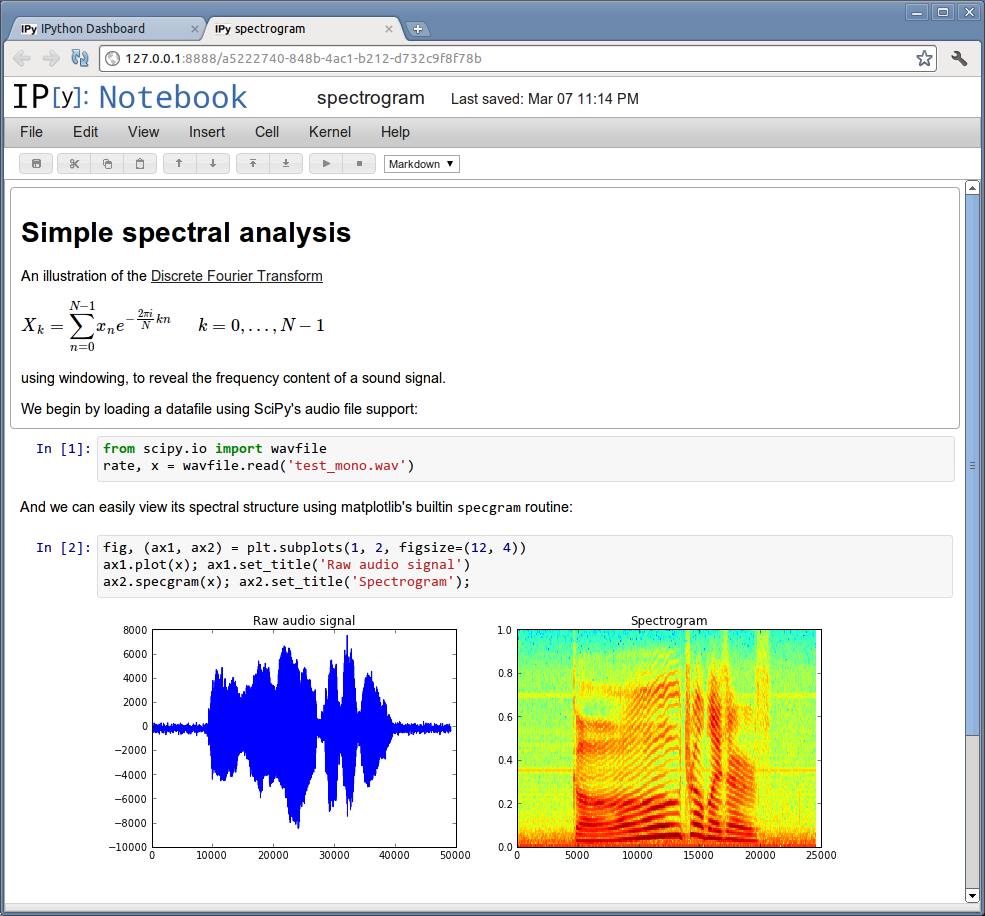
\includegraphics[width=3.2in]{../fig/ipython-notebook-specgram.png}\par
  \end{centering}

  \caption{\label{fig:IPython-notebook}The web-based IPython Notebook combines
    explanatory text, mathematics, multimedia, code and the results from
    executing the code.}
\end{figure}

\section{Conclusion}

\lipsum[1]

\bibliographystyle{plain}
\bibliography{example}

\clearpage
\appendix

\section*{Appendix}

Below ...

%% begin.rcode  p1, eval=FALSE
%% end.rcode

Below ...

%% begin.rcode  p2, eval=FALSE
%% end.rcode

Below ...

%% begin.rcode  p3, eval=FALSE
%% end.rcode

\end{document} 
